%\documentclass[11pt]{article}  % for e-submission to ApJ
\documentclass[11pt]{NSF}  % for e-submission to ApJ

%\documentclass[12pt,preprint2]{aastex}  % for e-submission to ApJ - two column

%\documentclass[manuscript]{emulateapj}  % this makes everything look like ApJ

\usepackage{graphicx, natbib, color, bm, amsmath, epsfig}

%paper commands, for when not using aastex
\newcommand\physrep{Phys.~Rep.}
\newcommand\fcp{Fund.~Cosmic~Phys.}
\newcommand{\pre}{Phys Rev E}
\newcommand{\apj}{ApJ}
\newcommand{\apjs}{ApJS}
\newcommand{\aj}{AJ}
\newcommand{\aap}{A\&A}
\newcommand{\mnras}{MNRAS}
\newcommand{\araa}{ARA\&A}
\newcommand{\procspie}{Proc.SPIE}
\newcommand{\pasj}{PASJ}
\newcommand{\iaucirc}{IAU Circ.}
\newcommand{\aplett}{AP Letters}
\newcommand{\aaps}{AAPS}
\newcommand{\aapr}{AAPR}
\newcommand{\nat}{Nature}
\newcommand{\apjsupp}{ApJS}
\newcommand{\pasp}{PASP}
\newcommand{\apjl}{ApJL}
\newcommand\prl{Phys.~Rev.~Lett.}
\newcommand\apss{Ap\&SS}




%%%% PUT NEW COMMANDS AND DEFINITIONS HERE %%%%
\usepackage{graphicx, natbib, color, bm, amsmath, epsfig}

%
% Hijacked and hacked from aastex.cls
%
%\def\newblock{\hskip .11em\@plus.33em\@minus.07em}%

%\newcommand\plotone[1]{%
% \typeout{Plotone included the file #1}
% \centering
% \leavevmode
% \includegraphics[width={\eps@scaling\columnwidth}]{#1}%
%}
%\newcommand\plotone[1]{
% \includegraphics[width=3.0in]{#1}%
%}
%\let\tableline=\hline
%enzo commands
\newcommand\jcompphys{J.~Comput.~Phys}
\newcommand\physfluidsa{Phys.~Fluids~A}
\newcommand\physfluids{Phys.~Fluids}
\newcommand\physlettA{Phys.~Lett.~A}
\newcommand\jfm{J.~Fluid~Mech.}
\newcommand\ccm{Comput.~Phys.~Commun.}
\newcommand\jphysique{J.~Physique~I}
\newcommand\revmodphys{Rev.~Mod.~Phys.~}

%\newcommand\aap{\ref@jnl{A\&A}}% 
%\newcommand\prb{\ref@jnl{Phys.~Rev.~B}}% 
          % Physical Review B: Solid State 


\newcommand{\ratio}{\mathcal{R}}
\newcommand{\yt}{{\tt yt}}
\newcommand{\Lmax}{\ell_{\rm max}}
\newcommand{\enzo}{{\small Enzo}}
\newcommand{\menzo}{{EnzoMHD}}
\newcommand{\Menzo}{{EnzoMHD}}
\newcommand{\zeus}{{\small ZEUS}}
\newcommand{\Lbox}{L_{\rm box}}
\newcommand{\Nroot}{N_{\rm root}}
\newcommand{\K}{\,\rm K}
\newcommand{\dave}{DaveThena}
\newcommand{\grid}{{\tt grid}}

%\newcommand{\lct}[3]{\ensuremath{\epsilon_{#1,#2,#3}}}
\newcommand{\lct}[1]{\ensuremath{\epsilon_{#1}}}
%grid location commands.
\newcommand{\iph}{i + \frac{1}{2}}
\newcommand{\imh}{i - \frac{1}{2}}
\newcommand{\jph}{j + \frac{1}{2}}
\newcommand{\jmh}{j - \frac{1}{2}}
\newcommand{\kph}{k + \frac{1}{2}}
\newcommand{\kmh}{k - \frac{1}{2}}

\newcommand{\ipmh}{i \pm \frac{1}{2}}
\newcommand{\half}{\frac{1}{2}}
\newcommand{\quart}{\frac{1}{4}}
\newcommand{\tquart}{\frac{3}{4}}

%physics commands
\newcommand{\avir}{\ensuremath{\alpha_{\rm{vir}}}}
\newcommand{\mach}{\ensuremath{\mathcal{M}}}
\newcommand{\hmag}{\ensuremath{H_{\rm{M}}}}
\newcommand{\alfmach}{\ensuremath{\mathcal{M_{\rm{A}}}}}
%\newcommand{\msun}{\ensuremath{\rm{M}_\odot}}
\newcommand{\msun}{\ensuremath{M_\odot}}
\newcommand{\lsun}{\ensuremath{L_\odot}}
\newcommand{\rsun}{\ensuremath{R_\odot}}

\def\mch{\ensuremath{M_{\rm{Ch}}}}
\def\AD{{\rm{AD}}}

%math commands
\def\rms{\ensuremath{\rm{rms}}}
\newcommand{\pts}[1]{\emph{(#1 pts)}}
\newcommand{\dbd}[2]{\frac{ \partial #1 }{ \partial #2} }
\newcommand{\ddbd}[2]{\frac{ d #1 }{ d #2} }
\newcommand{\dDbD}[2]{\frac{ \mathrm{D} #1 }{ \mathrm{D} #2} }
\newcommand{\curl}{\nabla \times}
\newcommand{\divb}{\ensuremath{\nabla \cdot {\bvec}}}
\newcommand{\divv}{\ensuremath{\nabla \cdot {\vvec}}}
\newcommand{\divbo}{$\nabla \cdot {\bf B} = 0$}
\newcommand{\intd}[1]{\int_#1^{#1 + \Delta #1} }
\newcommand{\dt}{\Delta t}
\newcommand{\dx}{\Delta x}
\newcommand{\dy}{\Delta y}
\newcommand{\dz}{\Delta z}
\newcommand{\p}[1]{#1^\prime }
\newcommand{\pp}[1]{#1^{\prime \prime} }
\newcommand{\tff}{\ensuremath{t_{\rm{ff}}}}
\newcommand{\kkmin}{\ensuremath{k/k_{\rm{min}}}}
\newcommand{\kmax}{\ensuremath{k_{\rm{max}}}}

%dcc color commands
\definecolor{orange}{rgb}{1.        ,  0.54,  0}
\newcommand{\orange}[1]{\textcolor{orange}{#1}}

\newcommand{\gtt}[1]{\textcolor{green}{{\tt#1}}}
\newcommand{\red}[1]{\textcolor{red}{#1}}
\newcommand{\yellow}[1]{\textcolor{yellow}{#1}}
\newcommand{\blue}[1]{\textcolor{blue}{#1}}
\definecolor{meta}{rgb}{0.371,0.617,0.625} %cadet blue for
                                           %non-production worthy
                                           % discussion of the work
\newcommand{\meta}[1]{\textcolor{meta}{#1}}
\newcommand{\green}[1]{\textcolor{green}{#1}}
\newcommand{\aake}[1]{\textcolor{blue}{#1}}
\newcommand{\bld}[1]{\mathbf{#1}}

\def\here{\red{notes later}}
%\newcommand{\hilite}[1]{\textcolor{red}{#1}}
%\newcommand{\hilite}[1]{#1}

%\newcommand{\bold}[1]{{\bf #1}}
%the comment maker, dc: the first one will show all comments in green, 
%the second hides them all.
%\newcommand{\dc}[1]{\textcolor{green}{#1}}
\newcommand{\dc}[1]{}
%\newcommand{\dc}[1]{#1}
%\def\bvec{\ensuremath{\vec{B}}}
%\def\vvec{\ensuremath{\vec{v}}}
\def\Bvec{\ensuremath{{\bf B}}}
\def\Jvec{\ensuremath{{\bf J}}}
\def\Avec{\ensuremath{{\bf A}}}
\def\bvec{\ensuremath{{\bf b}}}
\def\vvec{\ensuremath{{\bf v}}}
\def\uvec{\ensuremath{{\bf u}}}
\def\rvec{\ensuremath{{\bf r}}}
\def\xvec{\ensuremath{{\bf x}}}
\def\kvec{\ensuremath{{\bf k}}}
\def\Omegavec{\ensuremath{{\bf \Omega}}}
\def\omegavec{\ensuremath{{\bf \omega}}}
%\newcommand{\BlockOut}[1]{}
\newcommand{\BlockOut}[1]{#1}
\newcommand{\imp}{\ensuremath{\implies}}
\newcommand{\question}[1]{\textcolor{red}{#1}}
\definecolor{pink}{rgb}{1.        ,  0.75294118,  0.79607843}
\definecolor{maroon}{rgb}{0.69019608,  0.18823529,  0.37647059}
\newcommand{\ToRead}[1]{\textcolor{maroon}{#1}}
\newcommand{\ToReadUrgent}[1]{\textcolor{red}{#1}}
\newcommand{\HaveRead}[1]{\textcolor{black}{#1}}
\newcommand{\Old}[1]{\textcolor{blue}{#1}}
\newcommand{\Scanned}[1]{\textcolor{meta}{#1}}
\newcommand{\dccnote}[1]{}
%\newcommand{\dccnote}[1]{\textcolor{red}{#1}}
\def\nn{\nonumber}

\newcommand{\get}[1]{\textcolor{red}{#1}}
\definecolor{gray}{rgb}{0.5,0.5,0.5}
\newcommand{\gray}[1]{\textcolor{gray}{#1}}
\newcommand{\clean}[1]{\textcolor{gray}{#1}}
\newcommand{\ToDo}[1]{\textcolor{red}{#1}}
\def\etal{{\sl et al.}}

%chemistry commands
\newcommand{\Htwo}{\ensuremath{\rm{H}_2}}
\newcommand{\twelveco}{\ensuremath{^{12}\rm{CO}}}
\newcommand{\thirteenco}{\ensuremath{^{13}\rm{CO}}}

\newcommand{\mhdlabel}{{_{MHD}}}
\newcommand{\gravlabel}{{_{Grav}}}
\newcommand{\fclabel}{{_{fc}}}
\newcommand{\explabel}{{_{exp}}}
\newcommand{\sci}[1]{\ensuremath{\times {10^{#1}}}}
\newcommand{\percc}{\ensuremath{\rm{cm}^{-3}}}
\newcommand{\gcc}{\ensuremath{\rm{g}\ \rm{cm}^{-3}}}
\newcommand{\kms}{\ensuremath{\rm{km}\ \rm{s}^{-1}}}
\newcommand{\cms}{\ensuremath{\rm{cm}\ \rm{s}^{-1}}}
\newcommand{\cmperg}{\ensuremath{\rm{cm}^{2}\ \rm{g}^{-1} }}
\newcommand{\cmcmpers}{\ensuremath{\rm{cm}^2\ \rm{s}^{-1} }}
\def\muG{\ensuremath{\mu\rm{G}}}
\def\micron{\ensuremath{\mu\rm{m}}}
\def\alf{Alfv\' en}
\def\Alfvenic{Alfv\' enic}
\def\sa{super-Alfv\' enic}
\def\Sa{Super-Alfv\' enic}
\def\suba{sub-Alfv\' enic}
\def\Suba{Sub-Alfv\' enic}
\def\transa{trans-Alfv\' enic}
\def\Transa{Trans-Alfv\' enic}
\def\cs{\ensuremath{c_{\rm{s}}}}
\def\va{\ensuremath{v_{\rm{A}}}}
\def\sfrff{\ensuremath{{\rm SFR_{ff}}}}
%\def\velocity{\ensuremath{\vec{v}}}
%\def\magnetic{\ensuremath{\vec{B}}}
\def\velocity{\ensuremath{{\bf v}}}
\def\magnetic{\ensuremath{{\bf B}}}
\newcommand{\Fourier}[1]{\ensuremath{\tilde{#1}}}
\def\hfw{0.49}
\def\hw{0.49}
\def\fw{0.9}

\def\ssp{\def\baselinestretch{1.0}\large\normalsize}

\def\rhoc{\ensuremath{\rho_{\rm{c}}}}
\def\erf{\ensuremath{\rm{erf}}}


\def\SUtotal{2.9\sci{5}       }%cut from table1.
\def\tfinal{T_{\rm{final}}}
\def\suzu{\ensuremath{\rm{SU}_{\rm{zu}}}}
\def\nzones{N_{\rm{z},\ell}}
\newcommand{\Lund}{\ensuremath{\mathrm{S}}}
%\newcommand{\SUestimate}[1]{\textcolor{red}{#1}}
\newcommand{\SUestimate}[1]{#1}
\def\SUtotal{1.6\sci{5}       }                                                       
%\def\SUturb{1.8\sci{4}}
%\def\SUcore{1.2\sci{4}}
%\def\SUcmb{2.6\sci{4}}
%\def\SUgal{2.2\sci{3}}
%\def\DiskTurb{5.6\sci{3} Gb}
%\def\DiskCore{1.6\sci{5} Gb}
%\def\Diskcmb{1.7\sci{4} Gb}
%\def\Diskgal{1.1\sci{4} Gb}
%\def\StoreTotal{1.9\sci{5} Gb}
\def\nameTurbulence{\emph{turbulence}}
\def\nameTurbShort{\emph{turb}}
\def\nameCores{\emph{cores}}
\def\nameCMB{\emph{foregrounds}}
\def\nameGalaxies{\emph{galaxies}}
\def\suPerZoneUpTurbulence{\ensuremath{2.0\sci{-11}}}
\def\suPerZoneUpCores{\ensuremath{6.2\sci{-11}}}
\def\suPerZoneUpCMB{\ensuremath{6.2\sci{-11}}}
\def\suPerZoneUpGalaxies{\ensuremath{3\sci{-10}}}

\citestyle{aa}  % correct formatting for ApJ style files

\usepackage{aas_macros}
\begin{document}

\begin{centering}
\begin{LARGE}
Scaling Information for 

``Four Projects in Astrophysical Magnetohydrodynamics''
\end{LARGE}

David Collins, PI

\end{centering}


\pagestyle{plain}


In order to quantify the performance and scaling, and to select the number of
nodes to use for our jobs, we perform strong scaling studies for each of our four
projects.  For each suite, a fiducial simulation is performed
that targets the physics packages, root grid size, particle
count, and approximates the unpredictable adaptive mesh refinement (AMR)
structure of the production simulations.  
We perform a single time step on
the root grid, which takes many time steps on the subgrids. 
That time step is then repeated several times with an increasing number of
nodes.  Table \ref{table1} summarizes each of the suites, the total cost, the
physics package used, the AMR structure, the cost per update, and the number
of nodes to be used.



\begin{table}[h]
\begin{center}
    \caption{Summary of simulation projects.  The total node hours and disk
    usage are described in Section \ref{sec.plan}.  The physics packages used in
    eash project and
    adaptive mesh refinement (AMR) structure are described in Section
    \ref{sec.background}}
\begin{tabular}{lrrrr}\label{table1}
Name    &    Node Hours    &    Disk    &    Physics     &    AMR    \\
\hline
Turbulence    &   $1.8\sci{4}$  &   $5.6\sci{3}$  &    Hydro + Driving    &    None    \\
Cores         &   $1.2\sci{4}$  &   $1.6\sci{5}$  &    MHD + Gravity + Particles    &    4 levels, all space    \\
CMB           &   $2.6\sci{4}$  &   $1.7\sci{4}$  &    MHD + Driving    &    None    \\
Galaxies      &   $1.1\sci{4}$  &   $1.1\sci{4}$  &    MHD + Gravity + Cooling  &    8 level nest    \\
\hline
&    $6.6\sci{4}$    &    $1.9\sci{5}$   &        &        \\
\end{tabular}
\end{center}
\end{table}




The results can be seen in Figure \ref{fig.scaling}. Shown in the figure is \suzu, the number of
service units for the update of one cell, assuming 64 cores per node.  Each of
our four suites uses a different set of physics modules, which changes the cost
between suites.  Additionally they have different adaptive mesh refinement (AMR)
structure, which changes the overhead.  We discuss each suite below.

The quantity $\mu= core-hours/zone-update$, given perfect scaling, is
independent of the problem size and number of cores used.  It depends only on the
combination physics solvers.  The cost per zone-update is
$\suzu=\frac{\mu}{N_C/N_N}$, and the total cost $SU=\suzu N_Z N_U$, where $N_Z$ is the total number of
zones, and $N_U$ is the total number of updates.  $\suzu$\ also depends on the
number of cores per node, $N_C/N_N$, and all runs we use 64 cores per node.
Given perfect scaling, $\suzu$ is independent of
processor count.  However, our scaling is imperfect, and the optimal node number is
selected from  Figure \ref{fig.scaling}.

The blue line shows a set of 
fiducial simulations that use only the
relevant hydro solvers and gravity.  The hydro (or MHD) solver and gravity
solver are the most expensive part of the code, so we present their timing alone
as a baseline.
The simulations use either Piecewise
Parabolic Method \citep{Colella84} for the pure hydro turbulence simulations,
or the second order MHD scheme of \citep{Li08a} for the other three.  The points
in the blue line are, bottom to top, PPM, MHD, PPM+Gravity, MHD+Gravity.  

The orange line shows the scaling for the fiducial \nameTurbulence\
simulations.  These simulations will only use PPM and the turbulent driving
module, so only slightly more expensive than the baseline.  The
fiducial simulation is, as the production simulations will be, $1024^3$ root
grid with no AMR.
 We run on 4, 8, 16, and 32 nodes, using 64 cores per node.  The result is
$\suzu=2\sci{-11}$ on 4 cores, and $4\sci{-11}$ for 32 nodes.  Production runs
will run on 32
nodes, as the small increase in cost will be offset by the much shorter run
time.

The green curve shows the strong scaling for the fiducial \nameCores\
simulation.  This simulation has $512^3$ zones and $1024^3$ tracer particles.
On each of 4 levels, we refine a cubic region with volume based on the simulations
in \citep{Collins12}.  This package uses the gravity solver and MHD solvers as
well as the particle update machinery.
For this simulation, the density and pressure are uniform, which simplifies the
setup but does not affect the timing of the solver.  We will run these
simulations on 32 nodes as well, as the timing is favorable. 
Using 32 nodes will also give more peak memory, which is important as the memory
load during the simulation is far from constant as the mesh structure rebuilds
itself.

The red line shows the scaling for the \nameCMB\ simulations. The fiducial
simulation is also $1024^3$ and driving like the \nameTurbulence\ suite, but uses the MHD solver so is slightly more
expensive.  Due to the increased memory of the extra magnetic fields, we run on
8, 16, and 32 nodes.  We find $\suzu=2\sci{-11}-7\sci{-11}$.  
Again, we will use 32 nodes due to the short run times.

The final suite is the \nameGalaxies\ suite, shown in \red{purple}.  This suite
employs the most additional physics packages (including star formation,
cooling and heating, and chemistry).  The AMR structure
 is a nest of refinements, each about 1/8 of its
parent by volume (about half the length), that allows us to resolve both the disk and the circumgalactic medium.
It also gives roughly constant memory per level.
The fiducial simulations use 5 levels of refinement, rather than the target
9, but the amount of overhead relative to useful work doesn't change much going
from 5 to 9 levels  We use the same target root grid of 1.3 Mpc in physical
size and 256 zones on a side.  The AMR structure that Enzo produces is coincidentally 64 grid
patches per level, so we run our scaling study from 1 to 5 nodes with 64 cores
per node.     
This scaling is good, rising from $2\sci{-11}$ to $3\sci{-11}$. The refinement
structure will continue to 9 levels in the production runs, so we will use 9
nodes for the production simulations.


\begin{figure} \begin{center}
    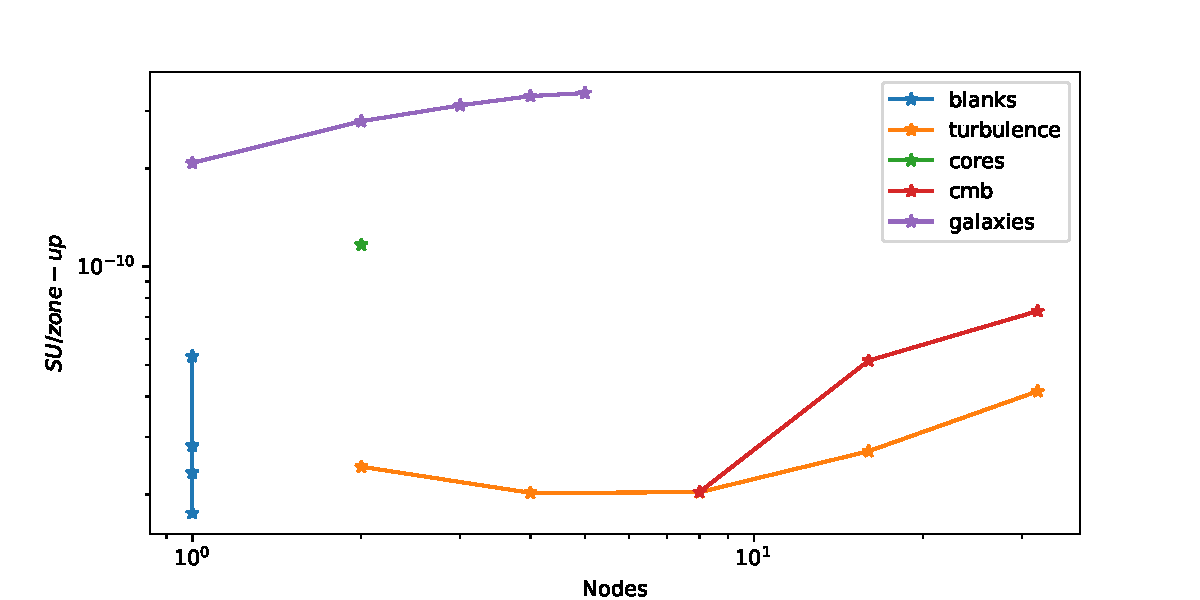
\includegraphics[width=0.99\textwidth]{figs/g47_zoneup.pdf}
\caption[ ]{The cost per zone-update for each of our simulation suites.  
Each fiducial simulation is nearly identical to the target production
simulations.
    }

\label{fig.scaling} \end{center} \end{figure}



\bibliographystyle{apj}
\bibliography{apj-jour,ms.bib}  % looks in ms.bib for bibliography info

\end{document}  


